\chapter*{CONSTRUCCIÓN DE UNA MONTAÑA RUSA}

\textbf{1)} Suponga que se le solicita diseñar el primer ascenso y descenso de un nuevo modelo de cohete. Después de estudiar fotografías de sus momentos rusos y precedentes, decide hacer la pendiente de ascenso 0.8 y la de descenso -1.6. Opta por conectar estos dos tramos rectos y es \( L(x) \) en pies para el tramo que parte del suelo y es \( f(x)= ax^2 + bx + c \), donde \( f'(x) \), su derivada, es \( 2ax + b \). Mediante el trabajo ya mencionado, puede calcular ambos coeficientes de dirección por lo que dispone que los segmentos para \( L \) y \( S \), sean tangentes al parabola en los puntos P y Q. Para simplificar las ecuaciones, decide situar el origen en P.

\begin{enumerate}[label=\alph*)]
	\item Suponga que la distancia horizontal entre P y Q es 100 pies. Escriba ecuaciones en \( a \), \( b \) y \( c \) que aseguren que le trayecto sea suave en los puntos de transición.
	\item Resuelva las ecuaciones del Inciso a) para \( a \), \( b \) y \( c \) para hallar una fórmula para \( f(x) \).
	\item Dibuje \( L_1 \) y \( L_2 \) para verificar gráficamente que las transiciones sean suaves.
	\item Encuentre la diferencia en elevación entre P y Q.
\end{enumerate}

\textbf{Inciso a)} Sea la coordenada \textbf{P} en el origen ya que es un punto conocido

$\therefore$ para la ecuación de la curva $f(x)$ pasa por el origen en el punto \textbf{P}, entonces $f(0)=0=a(0)^2 + b(0) + c \therefore c=0$

La derivada retorna la pendiente de la recta tangente en un punto de la curva y sabemos que el valor de la pendiente en el punto $P = 0.8$, por tanto:
\begin{align*}
	f'(x)|_{P(0,y)}=2ax+b|_{P(0,0)}=2a(0)+b=0.8 \\
	\therefore b=0.8
\end{align*}
Aplicando la misma lógica para el punto $Q(100,y(100))$ donde la pendiente $m_2=-1.6$:
\begin{align*}
	f'(x)|_{Q(100,y)}=2ax+b|_{Q(100,y)}=2a(100)+b= & -1.6 \\
	\implies 2(100)a+b=                            & -1.6 \\
	\therefore 200a+b=                             & -1.6 \\
\end{align*}

\textbf{Inciso b)} Hallar la fórmula f(x) resolviendo para a, b y c.
Por el inciso anterior sabemos que $b=0.8$ y $c=0$, entonces
\begin{align*}
	200a+0.8 & =-1.6             \\
	200a     & =-1.6-0.8         \\
	a        & =\frac{-2.4}{200} \\
	a        & =-0.012           \\
\end{align*}
$\therefore f(x)=-0.012x^2+0.8x$\\
$f'(x)=-0.024x+0.8$
\vspace*{1em}
\\
\textbf{Inciso c)} Dibular $L_1$ y $L_2$

Para dibujar las rectas neceistamos la derivada de la función $f(x)$, además sabemos que las ecuaciones de las rectas tangentes a cada punto de definen de la forma $y=(y(x_0)+y'(x_0)(x-x_0))$ para $L_1$ y $L_2$.

\begin{multicols}{2}
	\noindent
	\begin{align*}
		L_1= & (y(P_x)+y'(P_x)(x-P_x)), \;P(0,0) \\
		L_1= & 0+0.8(x-0)                        \\
		L_1= & 0.8x
	\end{align*}
	\columnbreak
	\begin{align*}
		L_2= & (y(Q_x)+y'(Q_x)(x-Q_x)), \;Q(100,y(100)) \\
		L_2= & -40-1.6(x-100)                           \\
		L_2= & -40-1.6x+160                             \\
		L_2= & 120-1.6x                                 \\
	\end{align*}
\end{multicols}

\begin{figure*}
	\centering
	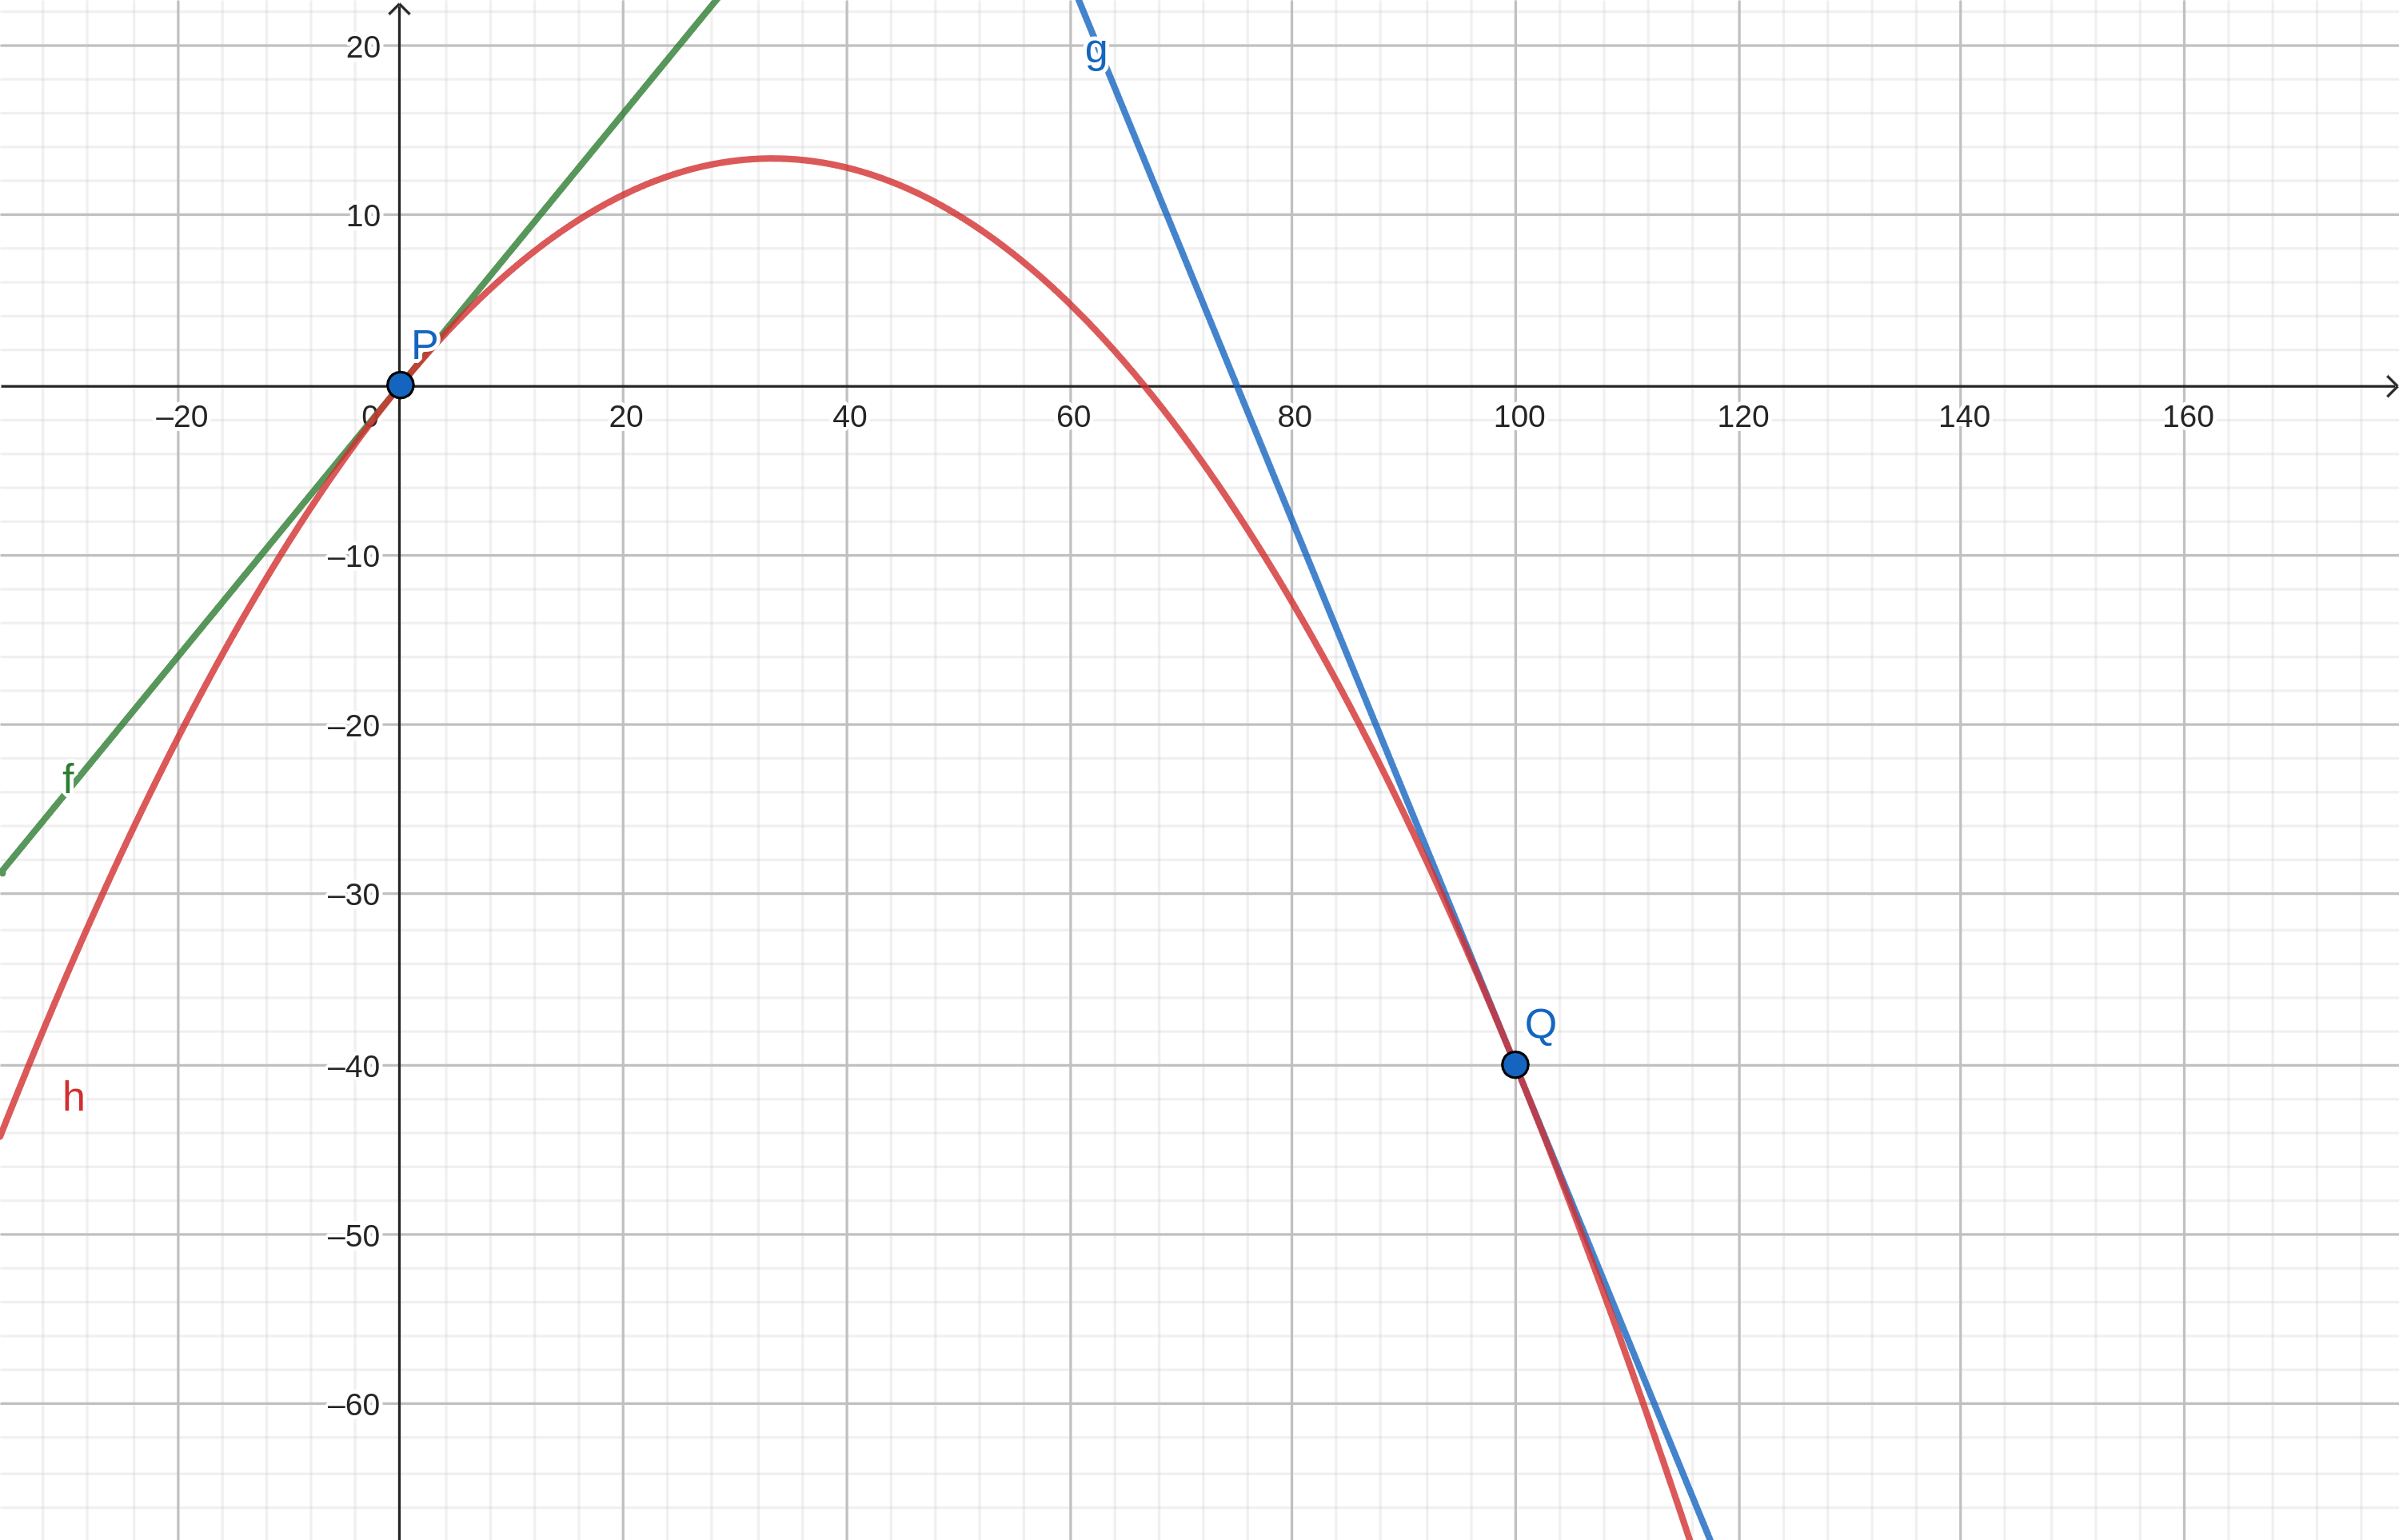
\includegraphics[height = 0.25\textheight]{recursos/geogebra-export.png}\par
	\caption*{Gráfica de las derivadas y la ecuación de la curva}
	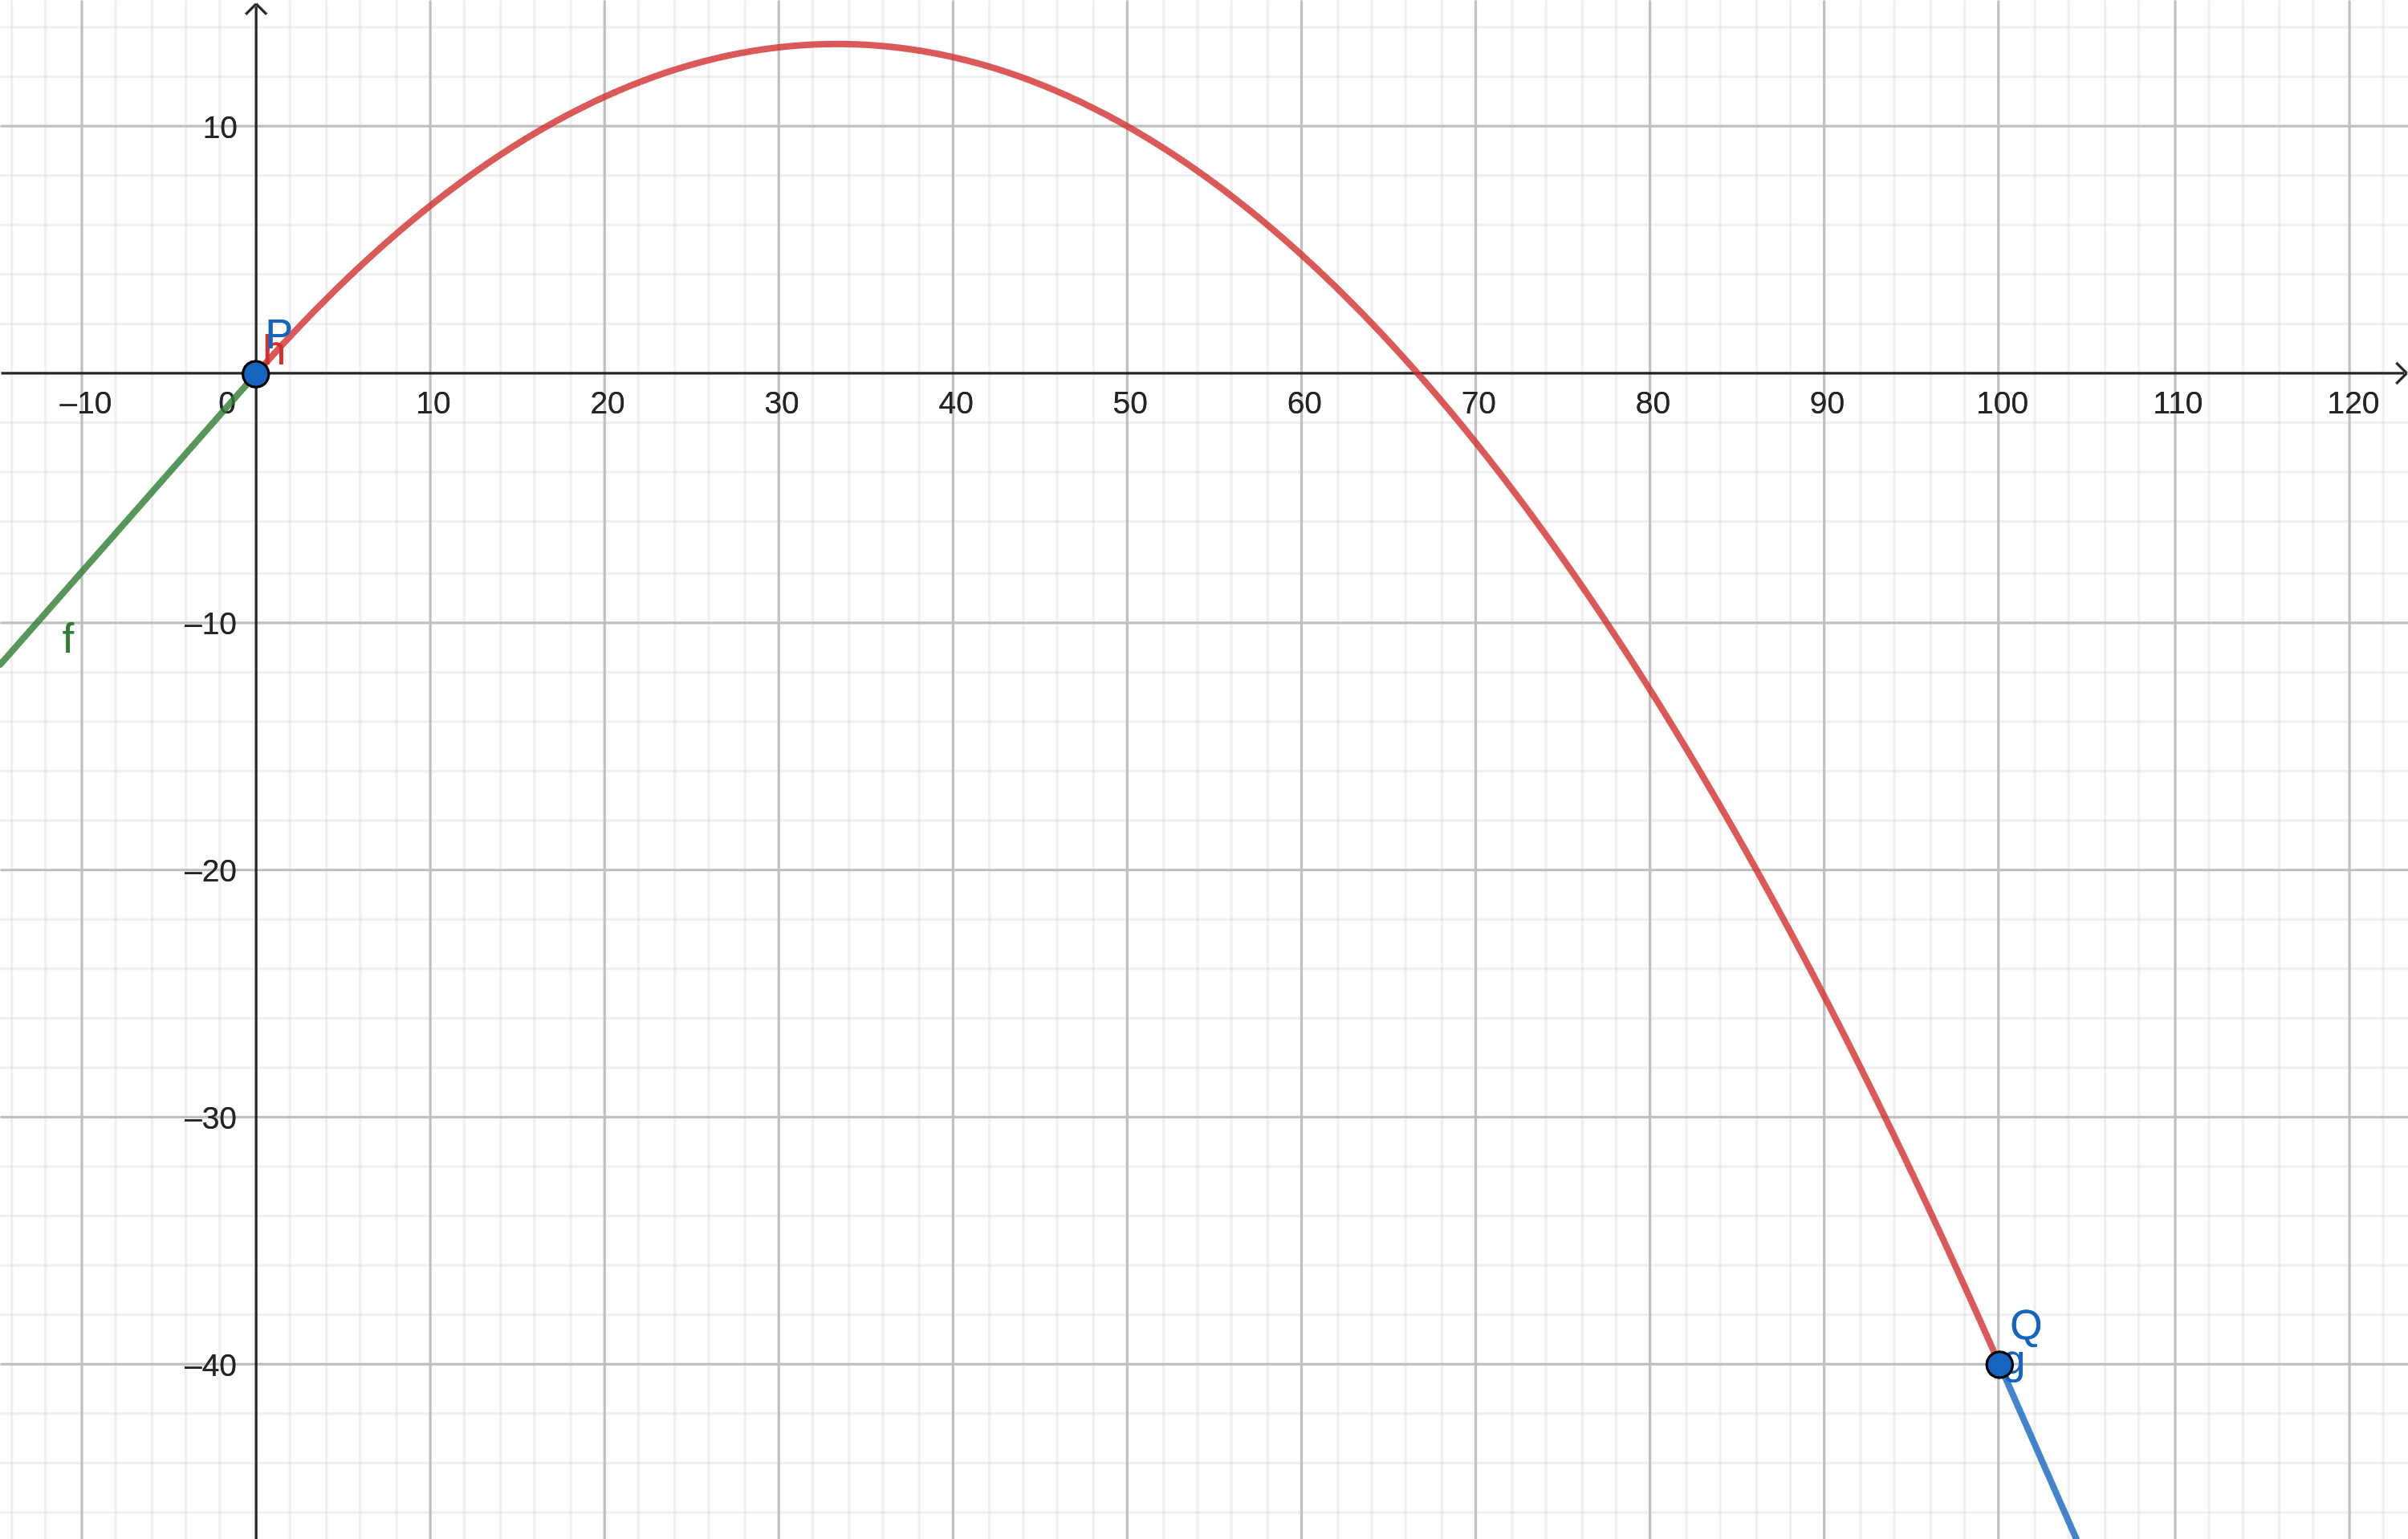
\includegraphics[height = 0.25\textheight]{recursos/geogebra-export5.png}\par
	\caption*{Gráfica donde se vizualizan las tranciones en los puntos de contacto P y Q}
\end{figure*}

\textbf{Inciso d)} La diferencia de elevación de cada punto está dado por el valor absoluto de la diferencia con respecto a el eje cordenado $y$ de los dos puntos

\begin{multicols}{2}
	\noindent
	\begin{align*}
		\text{Para el punto P} \\
		f(0)=0                 \\
	\end{align*}
	\columnbreak
	\begin{align*}
		\text{Para el }  & \text{punto Q en}  x = 100 \\
		f(100)           & =-0.012(100)^2+0.8(100)    \\
		f(100)           & =-0.012(100)^2+0.8(100)    \\
		f(100)           & =-120+80                   \\
		f(100)           & =-40                       \\
		\therefore Q(100 & ,-40)
	\end{align*}
\end{multicols}

$$\implies diferencia = |0-40|=40ft$$
\newpage
\textbf{2)} La solución del problema 1 puede parecer suave, pero es posible que no sienta lo suave debido a que la pieza definida como función [consistente en $L_1(x)$ para $x < 0$, $f (x)$ para $0 \leq x \leq 100$; y $L_2(x)$ para $x > 100$] no tiene una segunda derivada continua. Por consiguiente, usted decide mejorar su diseño utilizando una función cuadrática $q(x) = ax^2 + bx + c$ únicamente en el intervalo $10 \leq x \leq 90$ y conectarlo con las funciones lineales por medio de dos funciones cúbicas:
\begin{align*}
	g(x) & = kx^3 + lx^2 + mx + n \quad 0 \leq x < 10   \\
	h(x) & = px^3 + qx^2 + rx + s \quad 90 < x \leq 100
\end{align*}

\begin{enumerate}[label=\alph*)]
	\item Escriba un sistema de ecuaciones con 11 incógnitas que aseguren que las funciones y sus derivadas sean continuas en los puntos de transición.

	\item Resuelva las derivadas implicadas en un sistema algebraico computarizado para encontrar las fórmulas para \( g(x) \), \( q(x) \), y \( h(x) \).

	\item Dibuje $L_1$, $g$, $q$, $h$ y $L_2$ y compárelas con las gráficas del problema 1 anexo.
\end{enumerate}

\textbf{Inciso a)} Tenemos las funciones defindas en los siguientes intervalos
\begin{table}[!hbt]
	\begin{center}
		\begin{tabular}{| l | l | l | l | }
			\hline
			Función                       & Primera Derivada         & Segunda derivada & Intervalo       \\ \hline
			$L_1(x)=0.8x$                 & $L_1'(x)=0.8$            & $L_1 ''(x)=0$    & $(-\infty,0)$   \\
			$g(x) = kx^3 + lx^2 + mx + n$ & $g'(x) =3kx^2 + 2lx + m$ & $g''(x)=6kx+2l$  & $[0,10)$        \\
			$q(x) = ax^2 + bx + c$        & $q'(x) =2ax + b$         & $q''(x)=2a$      & $[10,90]$       \\
			$h(x) = px^3 + qx^2 + rx + s$ & $h'(x) =3px^2 + 2qx + r$ & $h''(x)=6px+2q$  & $(90,100]$      \\
			$L_2(x) = 120-1.6x$           & $L_2'(x)=-1.6$           & $L_2''(x)=0$     & $[100, \infty)$ \\ \hline
		\end{tabular}
		\caption{Tabla de funciones}
		\label{tab:la suma de los cilindros circunscritos como parabola}
	\end{center}
\end{table}

De acuderdo con lo establecido, las diferentes funciones deben ser iguales en los puntos de transición para garantizar que la entrada a la curva sea suave.

\begin{multicols}{4}
	\noindent
	\begin{align*}
		\text{Para } x = & 0        \\
		g(0)  =          & L_1(0)   \\
		g'(0) =          & L_1'(0)  \\
		g''(0)=          & L_1''(0) \\
	\end{align*}
	\columnbreak
	\begin{align*}
		\text{Para } x = & 10      \\
		g(10)  =         & q(10)   \\
		g'(10) =         & q'(10)  \\
		g''(10)=         & q''(10) \\
	\end{align*}
	\columnbreak
	\begin{align*}
		\text{Para } x = & 90       \\
		q(90)            & =h(90)   \\
		q'(90)           & =h'(90)  \\
		q''(90)          & =h''(90) \\
	\end{align*}
	\columnbreak
	\begin{align*}
		\text{Para } x = & 100        \\
		h(100)  =        & L_2(100)   \\
		h'(100) =        & L_2'(100)  \\
		h''(100)=        & L_2''(100) \\
	\end{align*}
\end{multicols}

Por lo tanto tenemos el siguiente sistema de ecuaciones de 11 incognitas.
\begin{align*}
	\text{Para }x=0                                      \\
	g(0)  = k(0)^3 + l(0)^2 + m(0) + n & = L_1(0)=0.8(0) \\
	g(0)  =  n                         & = L_1(0)=0      \\
	n                                  & = 0             \\
	g'(0) =3k(0)^2 + 2l(0) + m         & = L_1'(0)=0.8   \\
	g'(0) = m                          & = L_1'(0)=0.8   \\
	m                                  & = 0.8           \\
	g''(0)=6k(0)+2l                    & = L_1''(0)=0    \\
	g''(0)=2l                          & = L_1''(0)=0    \\
	2l                                 & = 0             \\
	l                                  & = 0             \\
	\therefore n=0; m=0.8; l=0                           \\
\end{align*}

\begin{align*}
	\text{Para }x=10                                                      \\
	g(10)  = k(10)^3 + l(10)^2 + m(10) + n & =q(10) = a(10)^2 + b(10) + c \\
	g(10)  = 1000k + 100l + 10m + n        & =q(10) = 100a + 10b + c      \\
	\implies 1000k + 100l + 10m + n        & =100a + 10b + c              \\
	g'(10) =3k(10)^2 + 2l(10) + m          & =q'(10) =2a(10) + b          \\
	g'(10) =3(100)k + 2(10)l + m           & =q'(10) =2(10)a + b          \\
	g'(10) =300k + 20l + m                 & =q'(10) =20a + b             \\
	\implies 300k + 20l + m                & =20a + b                     \\
	g''(10)=6k(10)+2l                      & =q''(10)=2a                  \\
	g''(10)=6(10)k+2l                      & =q''(10)=2a                  \\
	g''(10)=60k+2l                         & =q''(10)=2a                  \\
	\implies 60k+2l                        & =2a                          \\
\end{align*}
\begin{align*}
	\text{Para }x=90                                                     \\
	h(90) = p(90)^3 + q(90)^2 + r(90) + s & =q(90) = a(90)^2 + b(90) + c \\
	h(90) = 729000p + 8100q + 90r + s     & =q(90) = 8100a + 90b + c     \\
	\implies 729000p + 8100q + 90r + s    & = 8100a + 90b + c            \\
	h'(90) =3p(90)^2 + 2q(90) + r         & =q'(90) =2a(90) + b          \\
	h'(90) =3(8100)p + 2(90)q + r         & =q'(90) =2(90)a + b          \\
	h'(90) =24300p + 180q + r             & =q'(90) =180a + b            \\
	\implies 24300p + 180q + r            & =180a + b                    \\
	h''(90)=6p(90)+2q                     & =q''(90)=2a                  \\
	h''(90)=6(90)p+2q                     & =q''(90)=2a                  \\
	h''(90)=540p+2q                       & =q''(90)=2a                  \\
	\implies 540p+2q                      & =2a                          \\
\end{align*}

\begin{align*}
	\text{Para }x=100                                                    \\
	h(100) = p(100)^3 + q(100)^2 + r(100) + s & =L_2(100) = 120-1 6(100) \\
	h(100) = 1x10^6p + 1x10^4q + 100r + s     & =L_2(100) = 120-160      \\
	\implies 1x10^6p + 1x10^4q + 100r + s     & =-40                     \\
	h'(100) =3p(100)^2 + 2q(100) + r          & =L_2'(100)=-1.6          \\
	h'(100) =3(1x10^4)p + 200q + r            & =L_2'(100)=-1.6          \\
	\implies (3x10^4)p + 200q + r             & =-1.6                    \\
	h''(100)=6p(100)+2q                       & =L_2''(100)=0            \\
	h''(100)=600p+2q                          & =L_2''(100)=0            \\
	\implies 600p+2q                          & =0                       \\
\end{align*}

En resumen queremos resolver las ecuaciones para:
\begin{align*}
	n                                            & = 0   \\
	m                                            & = 0.8 \\
	2l                                           & = 0   \\
	-100a - 10b - c + 1000k + 100l + 10m + n     & =0    \\
	-20a - b +300k + 20l + m                     & = 0   \\
	- 2a + 60k+2l                                & =0    \\
	-8100a - 90b - c + 729000p + 8100q + 90r + s & = 0   \\
	-180a - b +24300p + 180q + r                 & = 0   \\
	1x10^6p + 1x10^4q + 100r + s                 & =-40  \\
	(3x10^4)p + 200q + r                         & =-1.6 \\
	600p+2q                                      & =0    \\
\end{align*}

\textbf{Inciso b)}Según el software \textbf{Matlab} el valor de cada incógnita es:
\begin{center}
	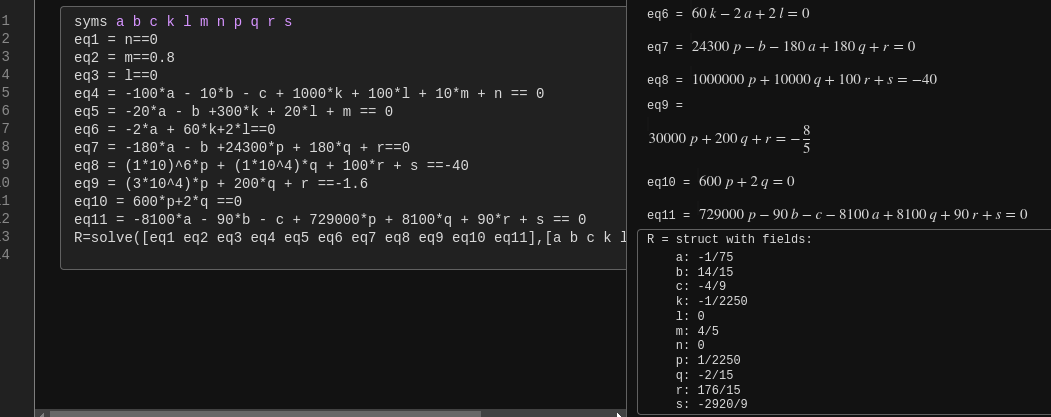
\includegraphics[height = 0.25\textheight]{recursos/Captura desde 2024-09-22 13-05-43.png}\par
\end{center}

$\implies$ Las formulas según los resultados son:
\begin{align}
	q(x) & =ax^2+bx+c                                   \\
	q(x) & =-\frac{1}{75}x^2+\frac{14}{15}x-\frac{4}{9}
\end{align}
\begin{align*}
	g(x) & =kx^3+lx^2+mx+n                         \\
	g(x) & =-\frac{1}{2250}x^3+0x^2+\frac{4}{5}x+0 \\
	g(x) & =-\frac{1}{2250}x^3+\frac{4}{5}x
\end{align*}
\begin{align*}
	h(x) & =px^3+qx^2+rx+s                                                   \\
	h(x) & =\frac{1}{2250}x^3-\frac{2}{15}x^2+\frac{176}{15}x-\frac{2920}{9} \\
\end{align*}

\textbf{Inciso c)} Las gráficas $L_1$, $g$, $q$, $h$ y $L_2$ y compárelas con las gráficas del problema 1 anexo.

\begin{figure*}
	\centering
	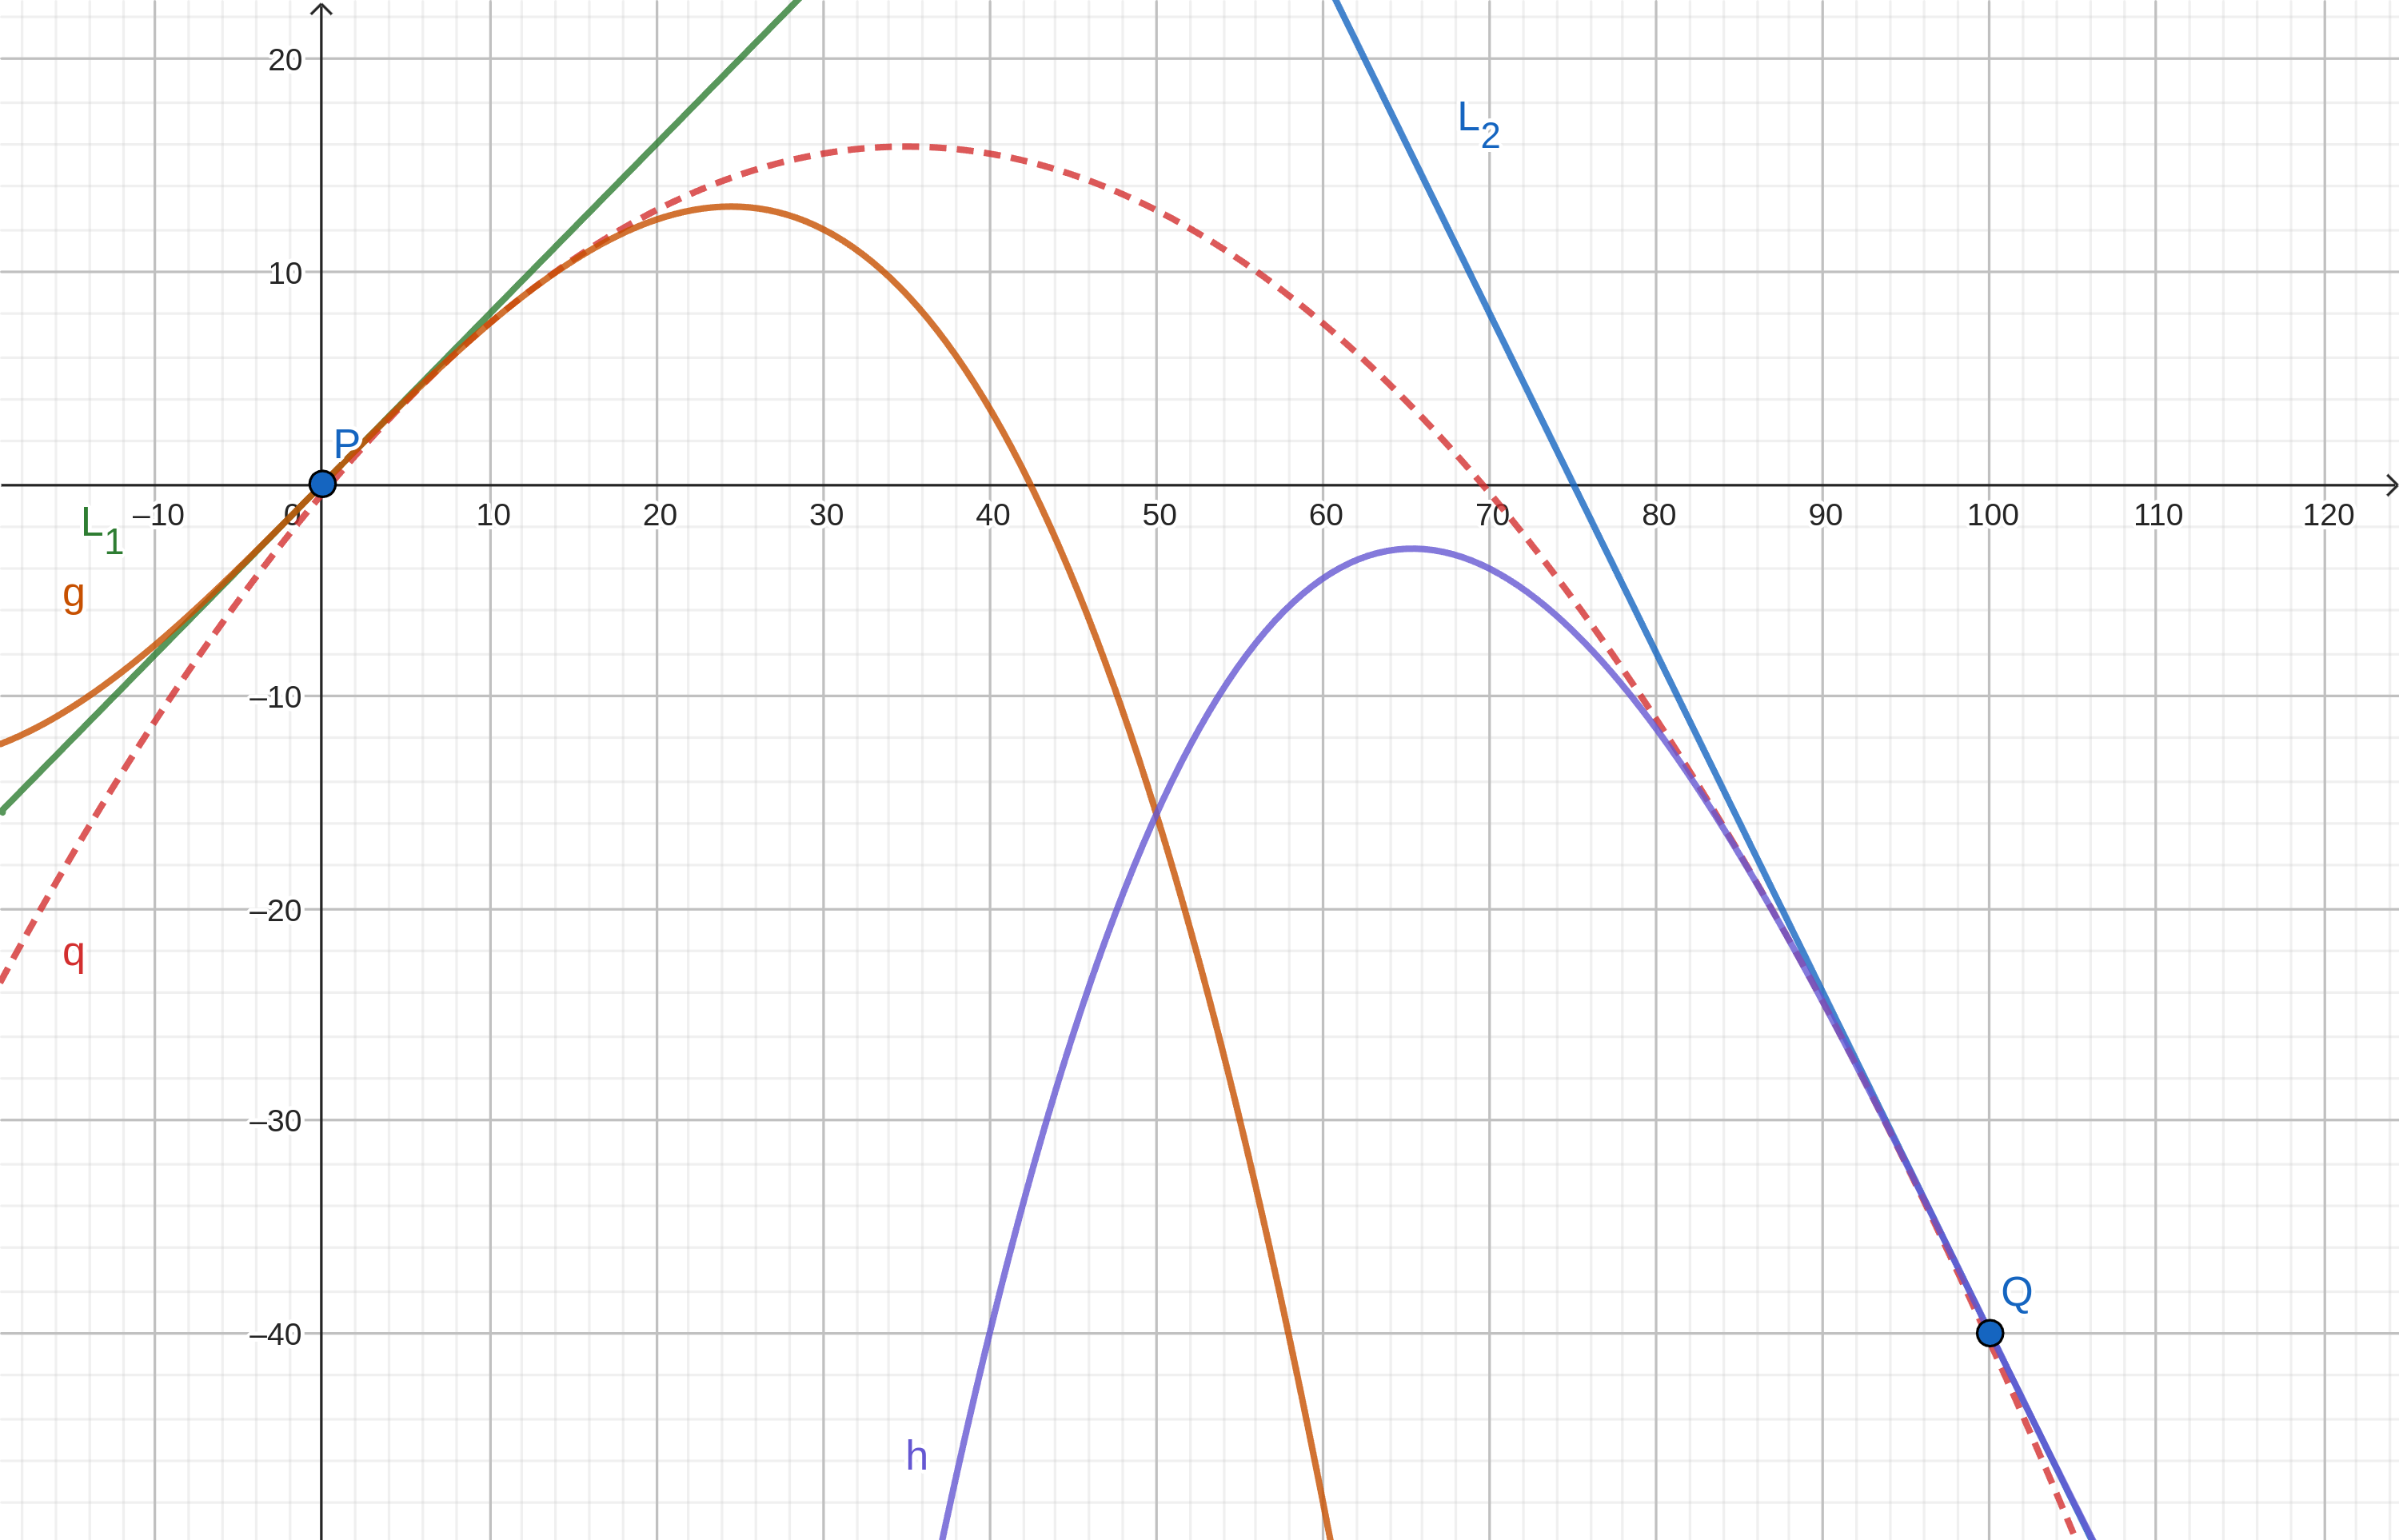
\includegraphics[height = 0.25\textheight]{recursos/geogebra-export1.png}\par
	\caption*{Las 5 ecuaciones completas que pasan por los mismos puntos de transición P y Q}
\end{figure*}

\begin{figure*}
	\centering
	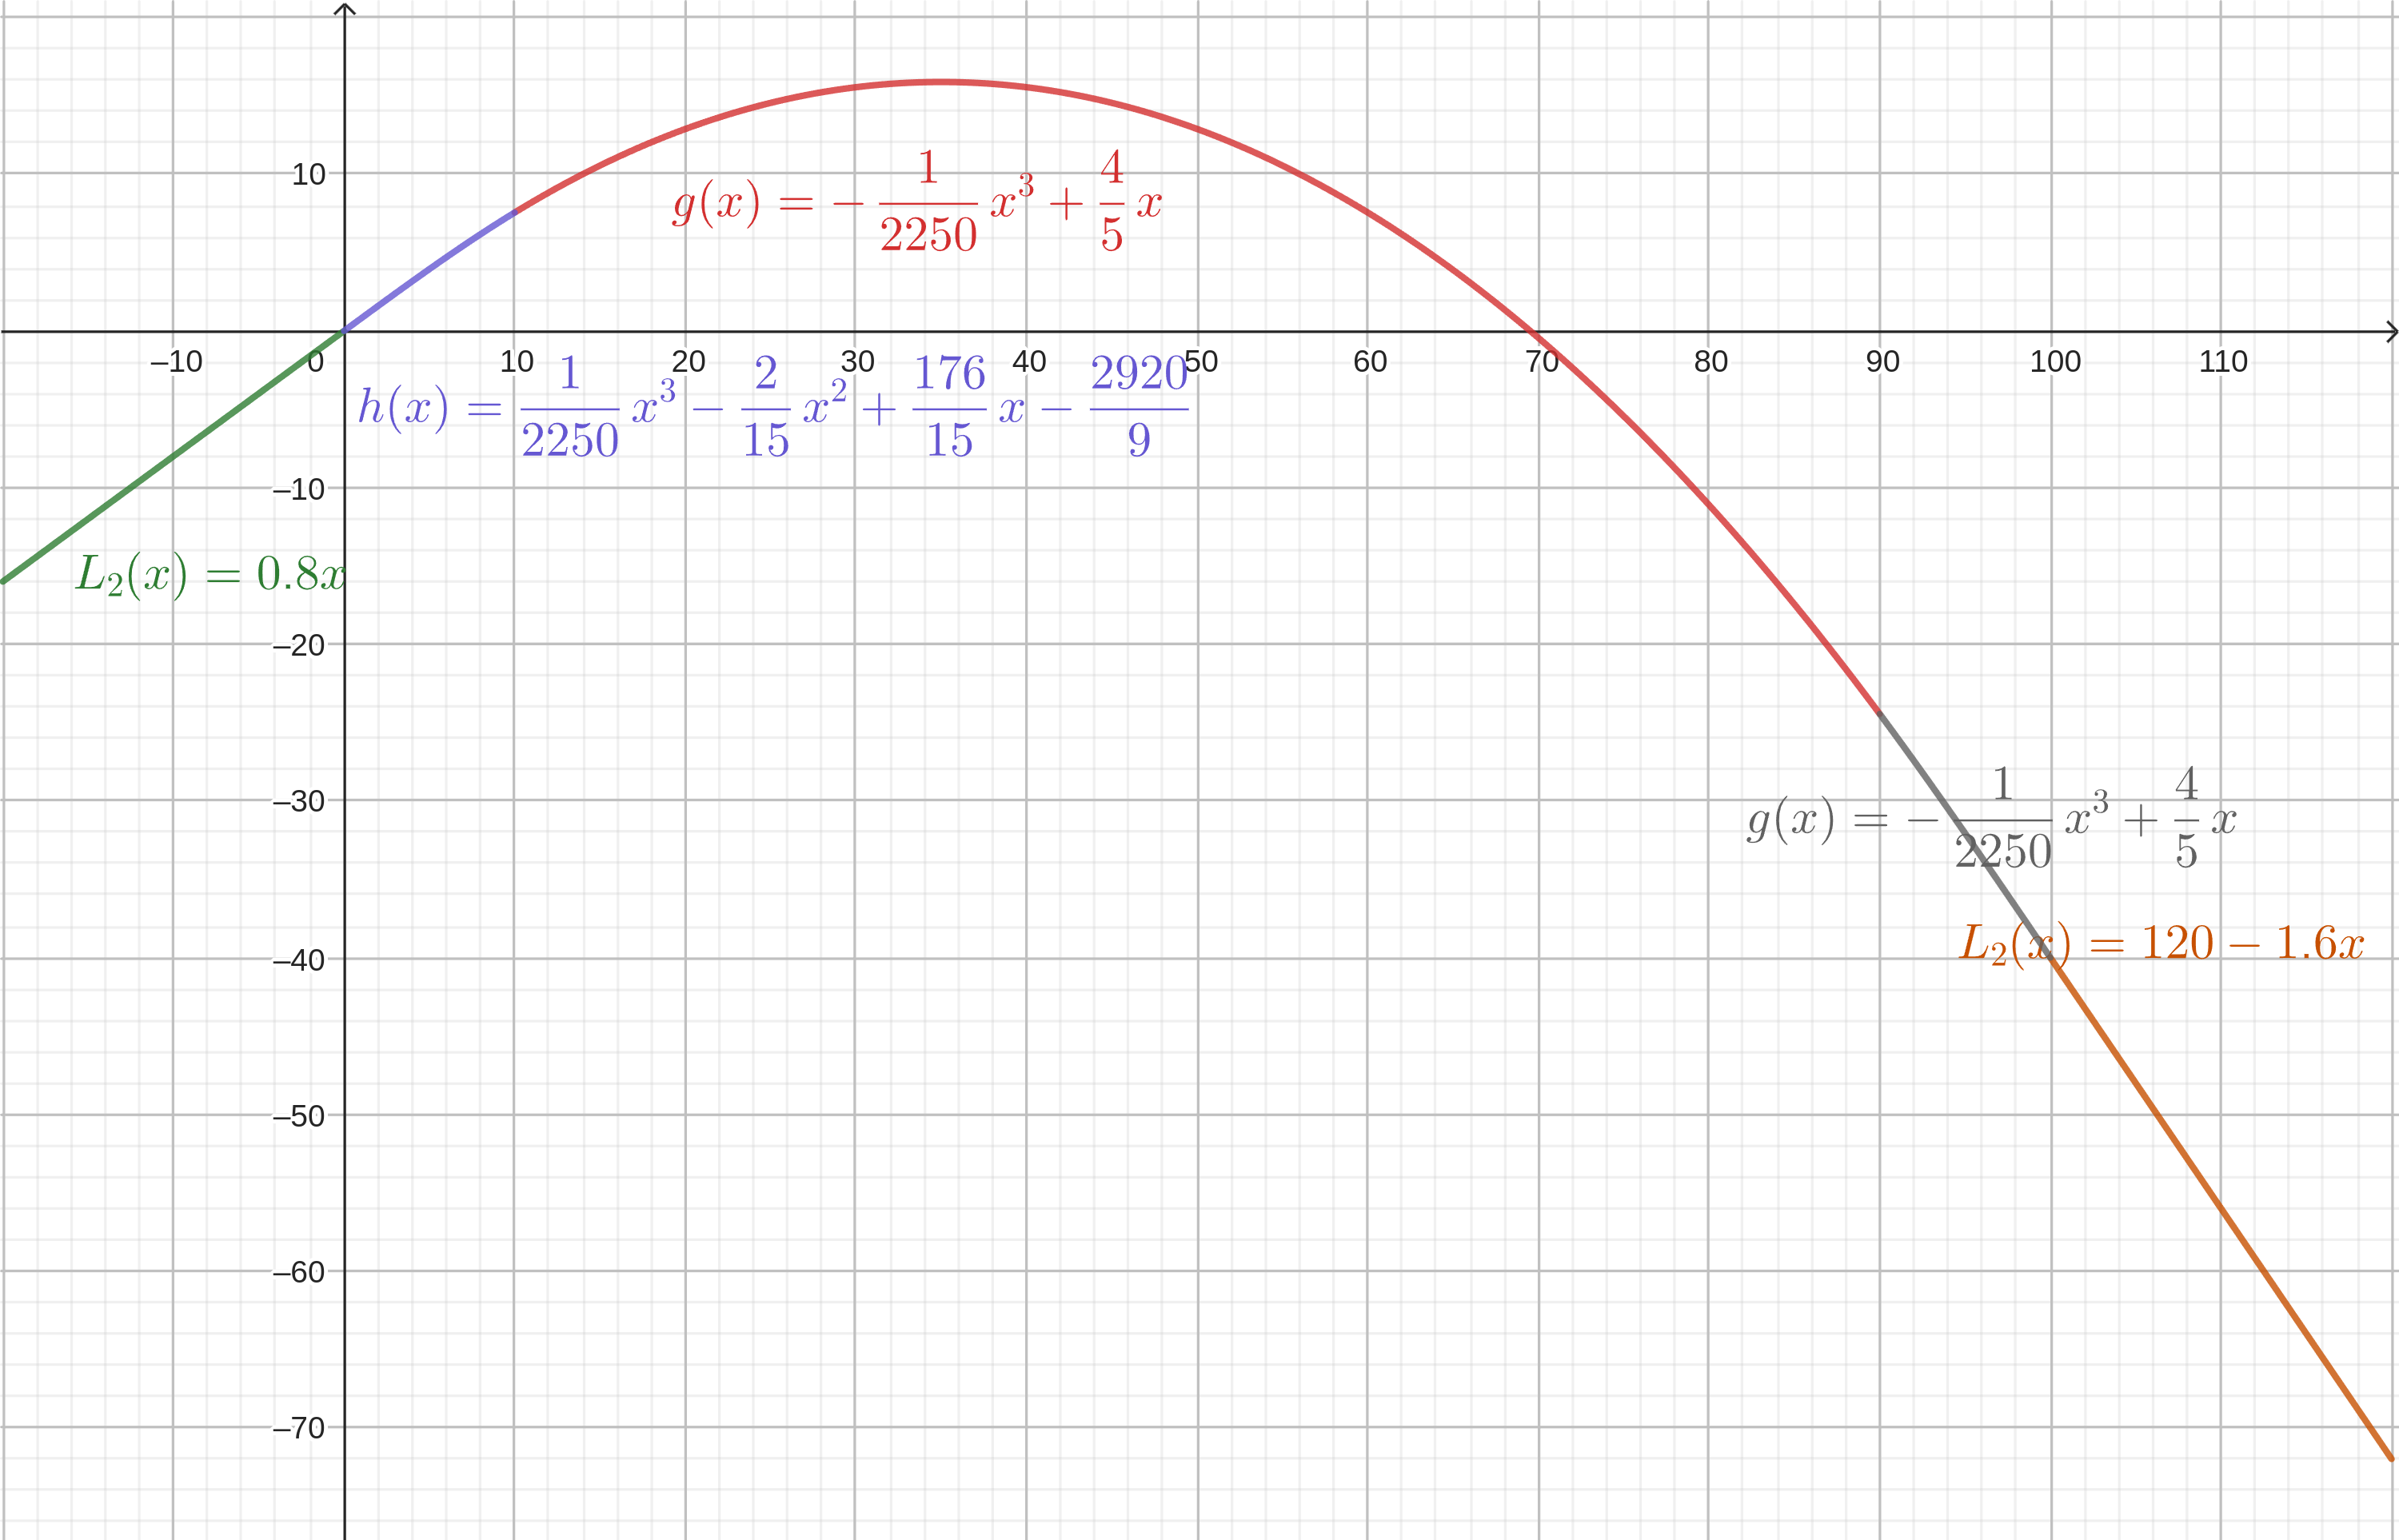
\includegraphics[height = 0.25\textheight]{recursos/geogebra-export2.png}\par
	\caption*{Las 5 ecuaciones de la parte dos del ejercicio con sus intervalos definidos para la construcción de la montaña Rusa.}
\end{figure*}
\begin{figure*}
	\centering
	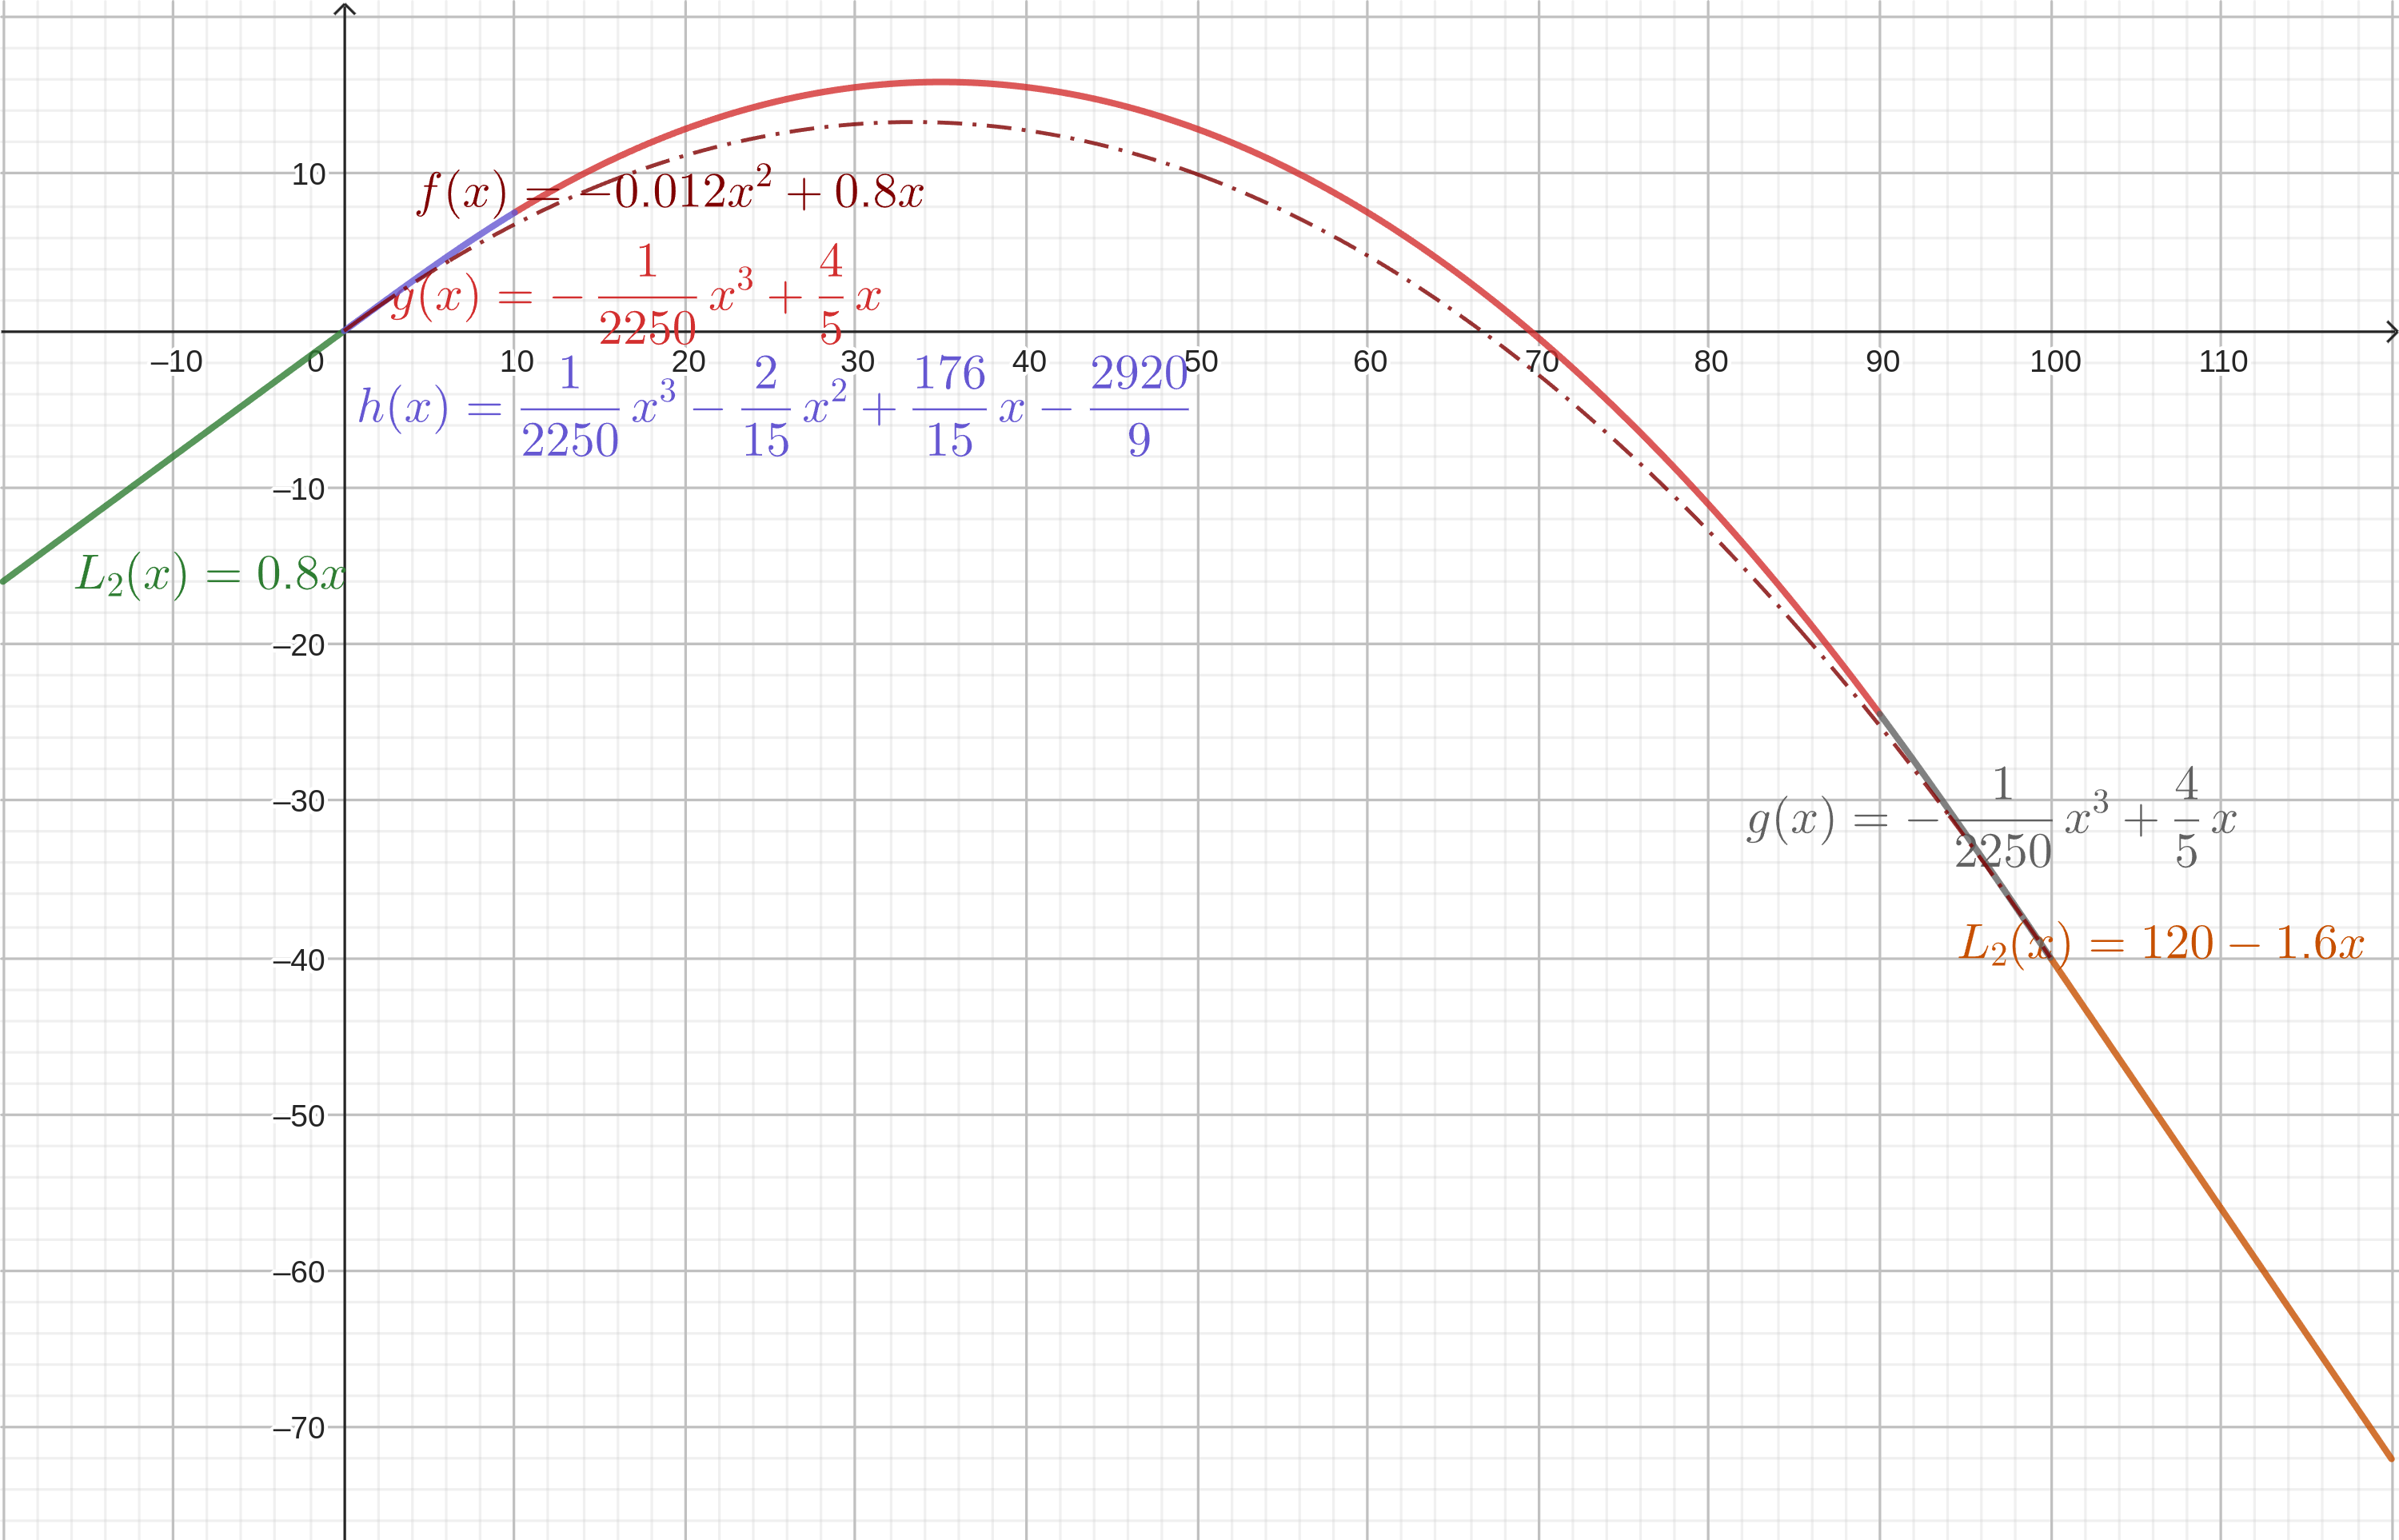
\includegraphics[height = 0.25\textheight]{recursos/geogebra-export3.png}\par
	\caption*{Comparación con la función generada en la primera parte del ejercicio mostrando, la segunda forma una continuidad más suave en cada transición}
\end{figure*}


